\documentclass[12pt]{article}
 
\usepackage[margin=1in]{geometry}
\usepackage{amsmath,amsthm,amssymb}
\usepackage{mathtools}
\DeclarePairedDelimiter{\ceil}{\lceil}{\rceil}
%\usepackage{mathptmx}
\usepackage{accents}
\usepackage{comment}
\usepackage{graphicx}
\usepackage{IEEEtrantools}
 \usepackage{float}
 
\newcommand{\N}{\mathbb{N}}
\newcommand{\Z}{\mathbb{Z}}
\newcommand{\R}{\mathbb{R}}
\newcommand{\Q}{\mathbb{Q}}
\newcommand*\conj[1]{\bar{#1}}
\newcommand*\mean[1]{\bar{#1}}
\newcommand\widebar[1]{\mathop{\overline{#1}}}


\newcommand{\cc}{{\mathbb C}}
\newcommand{\rr}{{\mathbb R}}
\newcommand{\qq}{{\mathbb Q}}
\newcommand{\nn}{\mathbb N}
\newcommand{\zz}{\mathbb Z}
\newcommand{\aaa}{{\mathcal A}}
\newcommand{\bbb}{{\mathcal B}}
\newcommand{\rrr}{{\mathcal R}}
\newcommand{\fff}{{\mathcal F}}
\newcommand{\ppp}{{\mathcal P}}
\newcommand{\eps}{\varepsilon}
\newcommand{\vv}{{\mathbf v}}
\newcommand{\ww}{{\mathbf w}}
\newcommand{\xx}{{\mathbf x}}
\newcommand{\ds}{\displaystyle}
\newcommand{\Om}{\Omega}
\newcommand{\dd}{\mathop{}\,\mathrm{d}}
\newcommand{\ud}{\, \mathrm{d}}
\newcommand{\seq}[1]{\left\{#1\right\}_{n=1}^\infty}
\newcommand{\isp}[1]{\quad\text{#1}\quad}

\DeclareMathOperator{\imag}{Im}
\DeclareMathOperator{\re}{Re}
\DeclareMathOperator{\diam}{diam}
\DeclareMathOperator{\Tr}{Tr}

\def\upint{\mathchoice%
    {\mkern13mu\overline{\vphantom{\intop}\mkern7mu}\mkern-20mu}%
    {\mkern7mu\overline{\vphantom{\intop}\mkern7mu}\mkern-14mu}%
    {\mkern7mu\overline{\vphantom{\intop}\mkern7mu}\mkern-14mu}%
    {\mkern7mu\overline{\vphantom{\intop}\mkern7mu}\mkern-14mu}%
  \int}
\def\lowint{\mkern3mu\underline{\vphantom{\intop}\mkern7mu}\mkern-10mu\int}




\newenvironment{theorem}[2][Theorem]{\begin{trivlist}
\item[\hskip \labelsep {\bfseries #1}\hskip \labelsep {\bfseries #2.}]}{\end{trivlist}}
\newenvironment{lemma}[2][Lemma]{\begin{trivlist}
\item[\hskip \labelsep {\bfseries #1}\hskip \labelsep {\bfseries #2.}]}{\end{trivlist}}
\newenvironment{exercise}[2][Exercise]{\begin{trivlist}
\item[\hskip \labelsep {\bfseries #1}\hskip \labelsep {\bfseries #2.}]}{\end{trivlist}}
\newenvironment{problem}[2][Problem]{\begin{trivlist}
\item[\hskip \labelsep {\bfseries #1}\hskip \labelsep {\bfseries #2.}]}{\end{trivlist}}
\newenvironment{question}[2][Question]{\begin{trivlist}
\item[\hskip \labelsep {\bfseries #1}\hskip \labelsep {\bfseries #2.}]}{\end{trivlist}}
\newenvironment{corollary}[2][Corollary]{\begin{trivlist}
\item[\hskip \labelsep {\bfseries #1}\hskip \labelsep {\bfseries #2.}]}{\end{trivlist}}

\newenvironment{solution}{\begin{proof}[Solution]}{\end{proof}}
 
\begin{document}
 
% --------------------------------------------------------------
%                         Start here
% --------------------------------------------------------------
\title{Math 115A Midterm}
\author{Ethan Martirosyan}
\date{\today}
\maketitle
\hbadness=99999
\hfuzz=50pt
\section*{Problem 1}
\subsection*{Part (i)}
\begin{figure}[H]
\centering
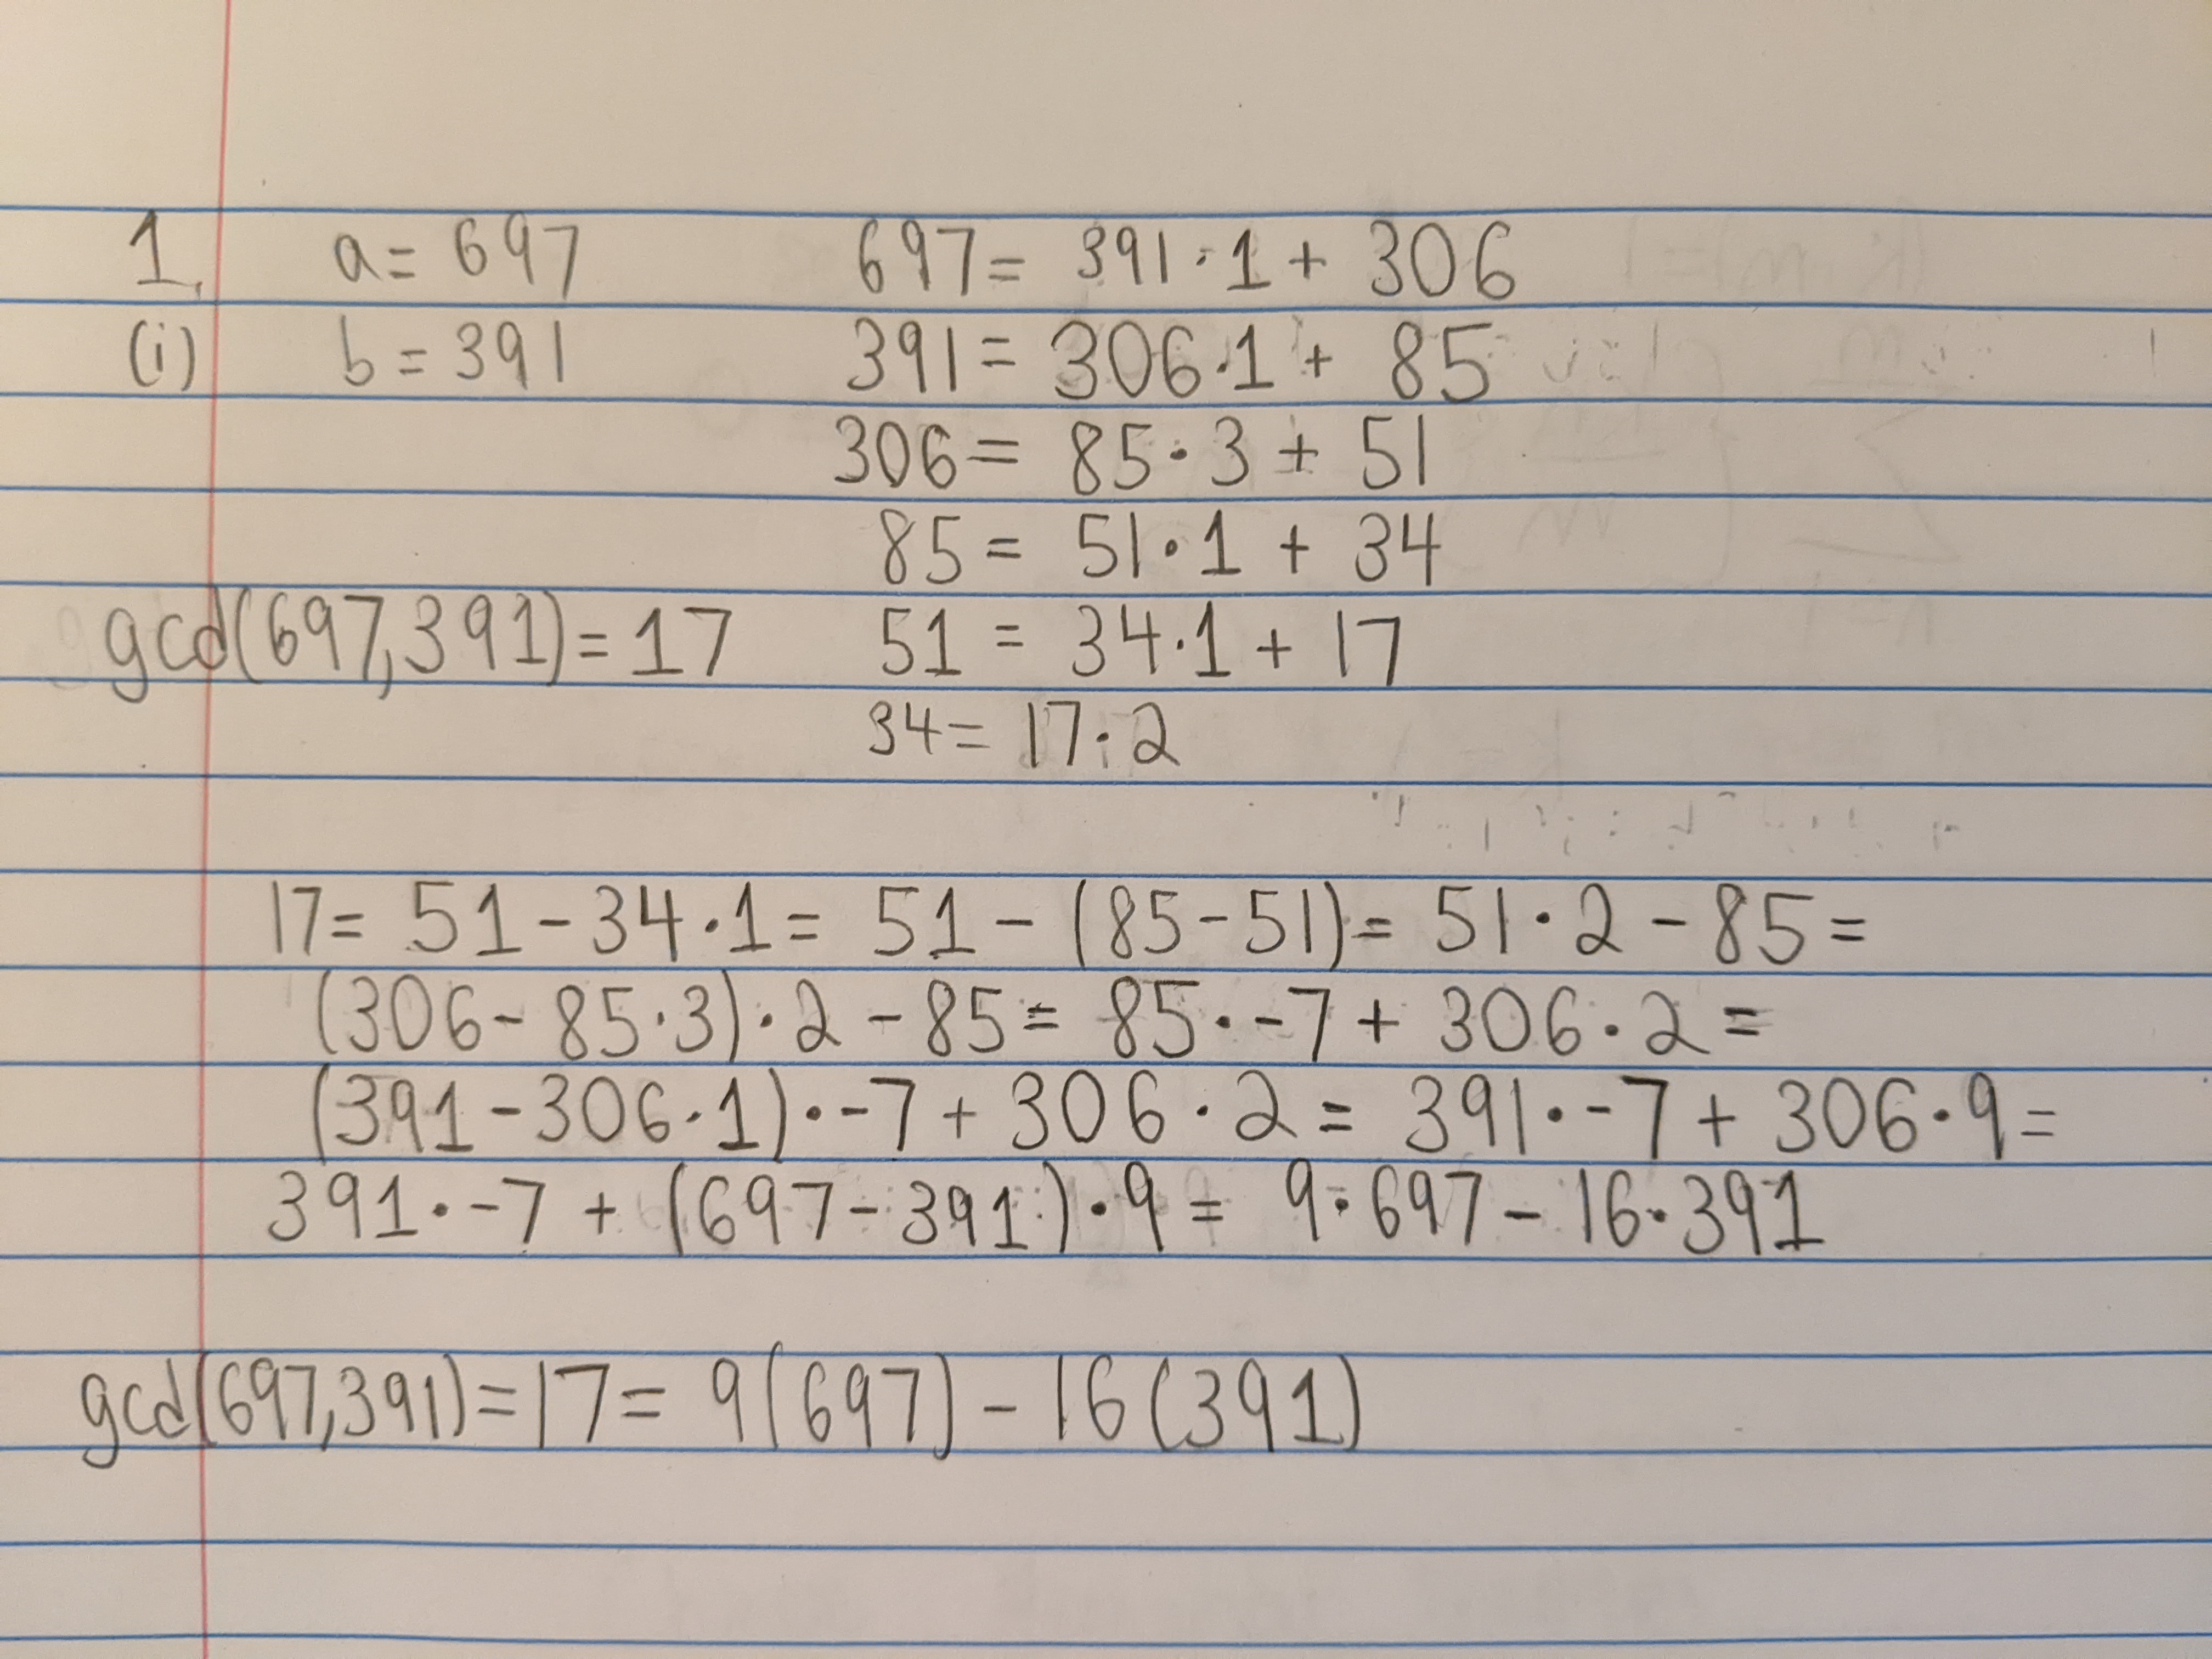
\includegraphics[width=\textwidth]{Problem1Image1}
\end{figure}
\newpage
\subsection*{Part (ii)}
 \begin{figure}[H]
\centering
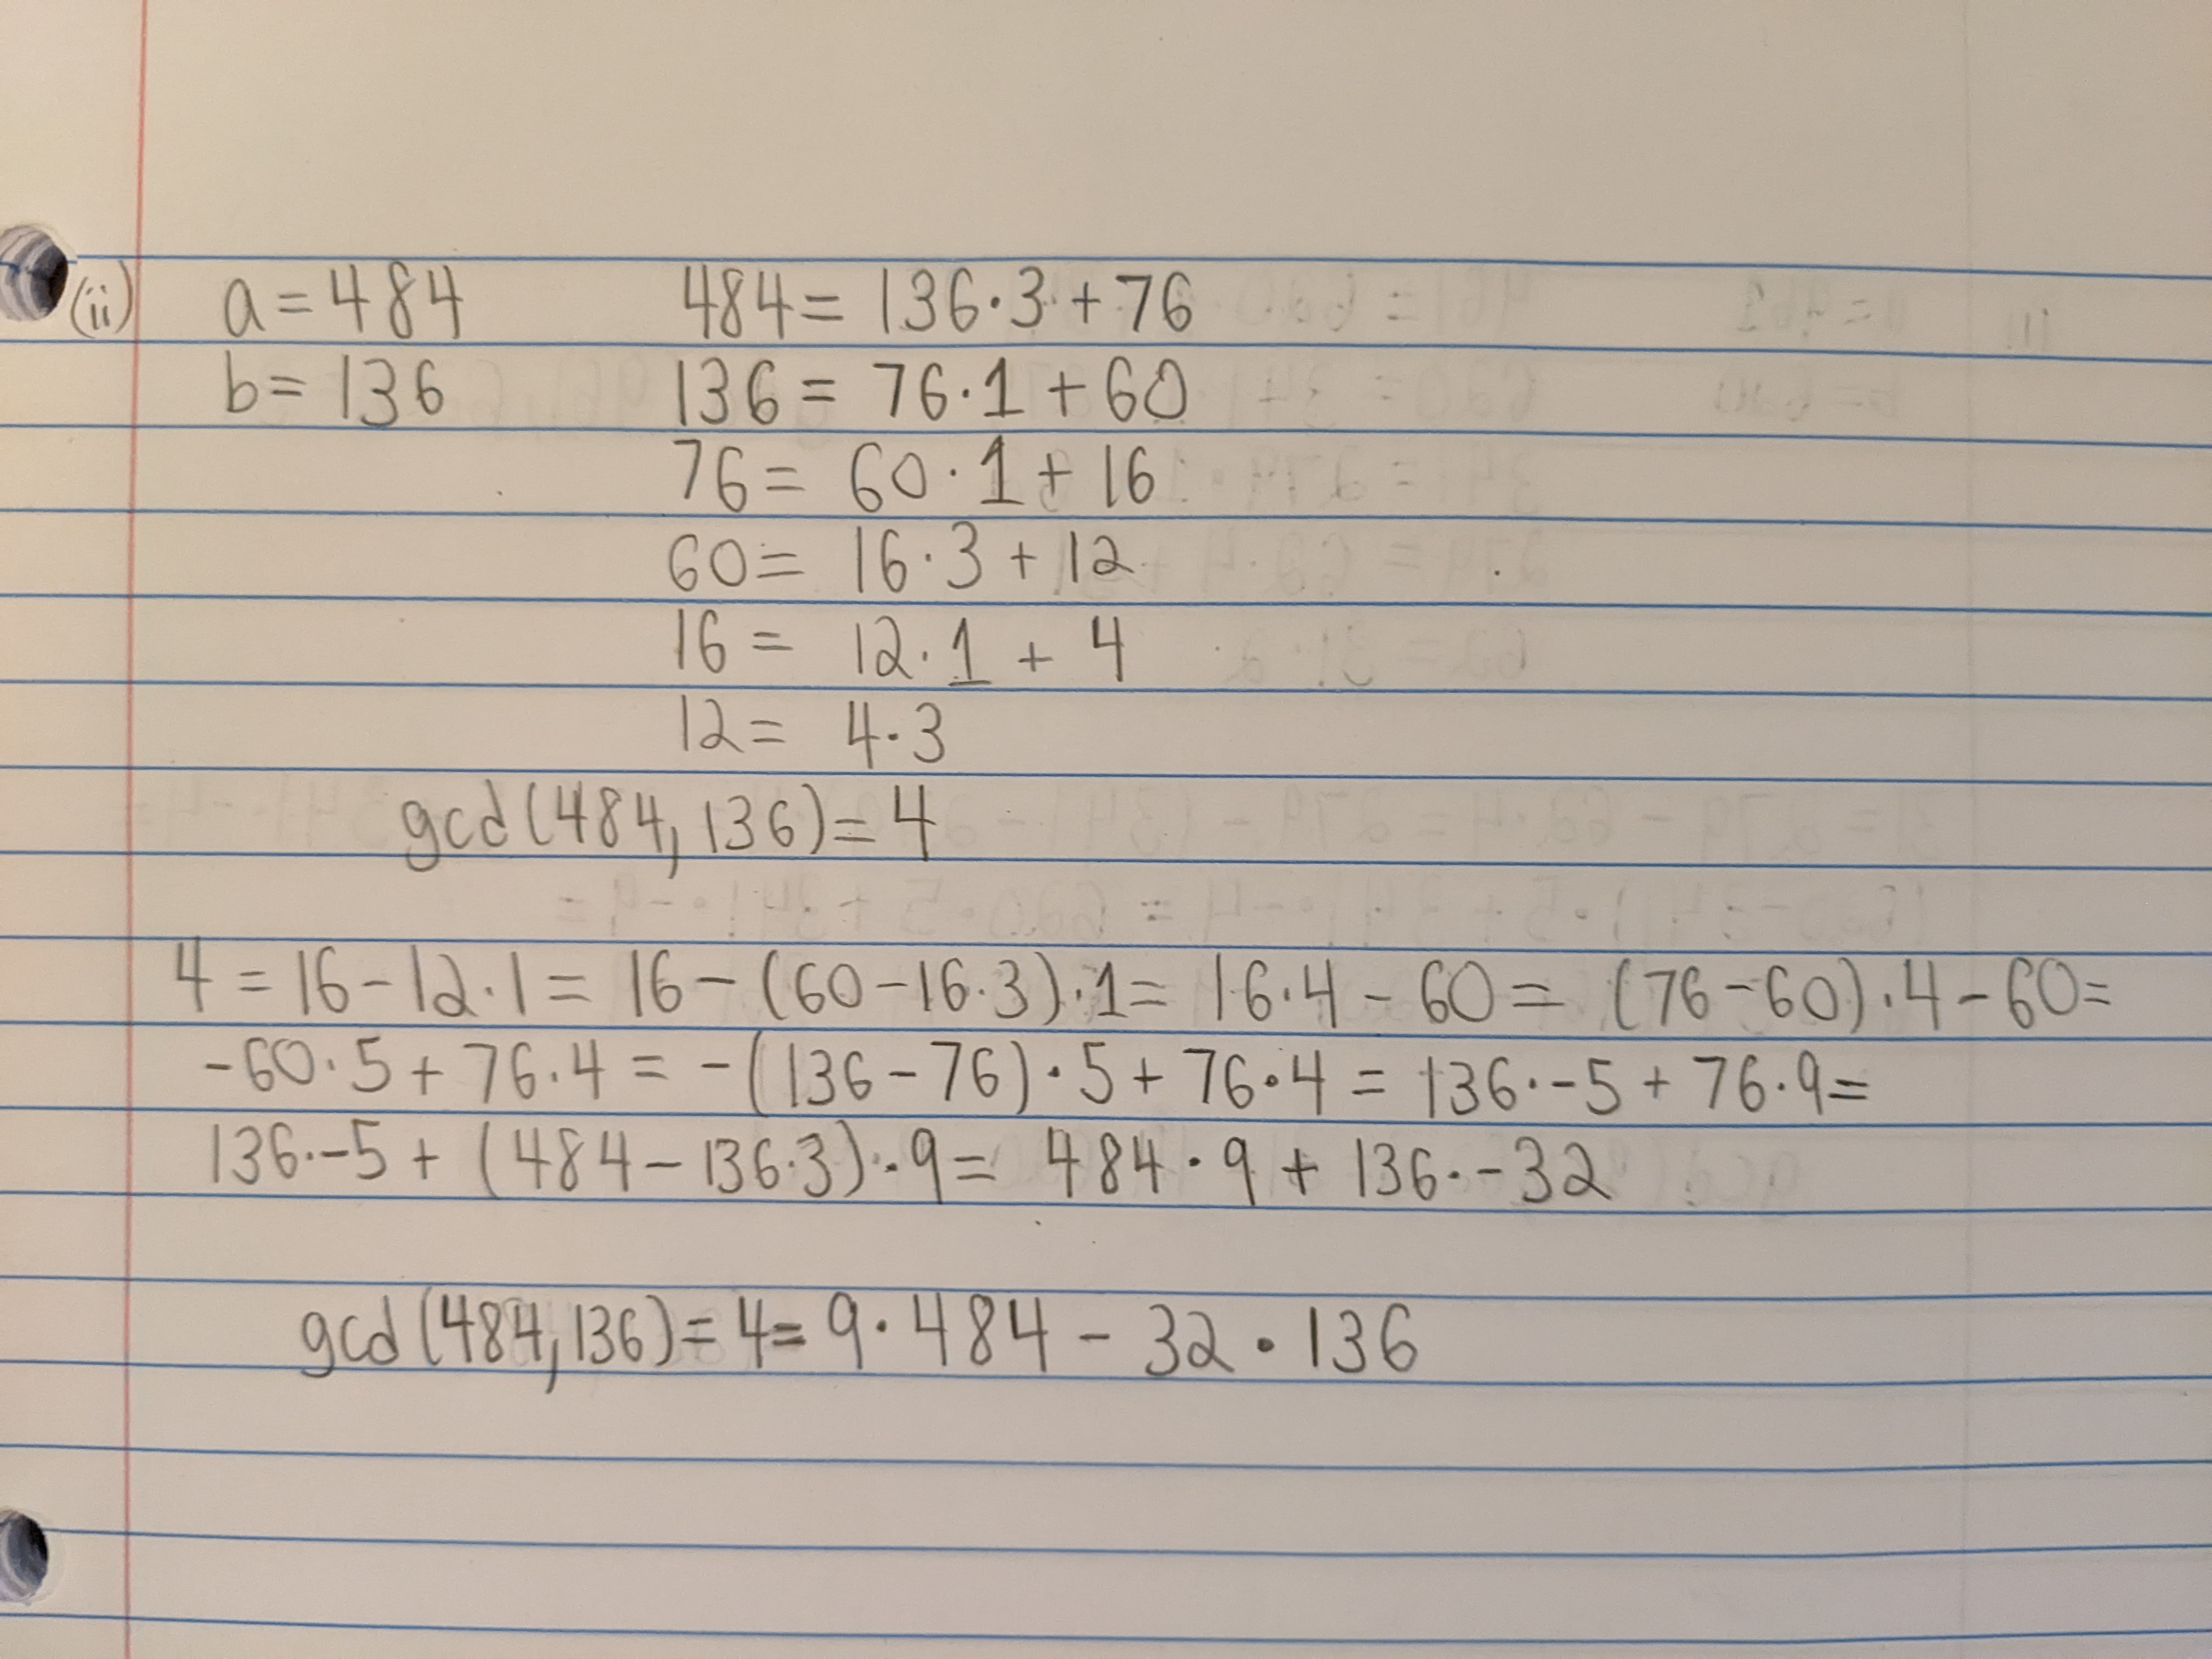
\includegraphics[width=\textwidth]{Problem1Image2}
\end{figure}
\newpage
\subsection*{Part (iii)}
 \begin{figure}[H]
\centering
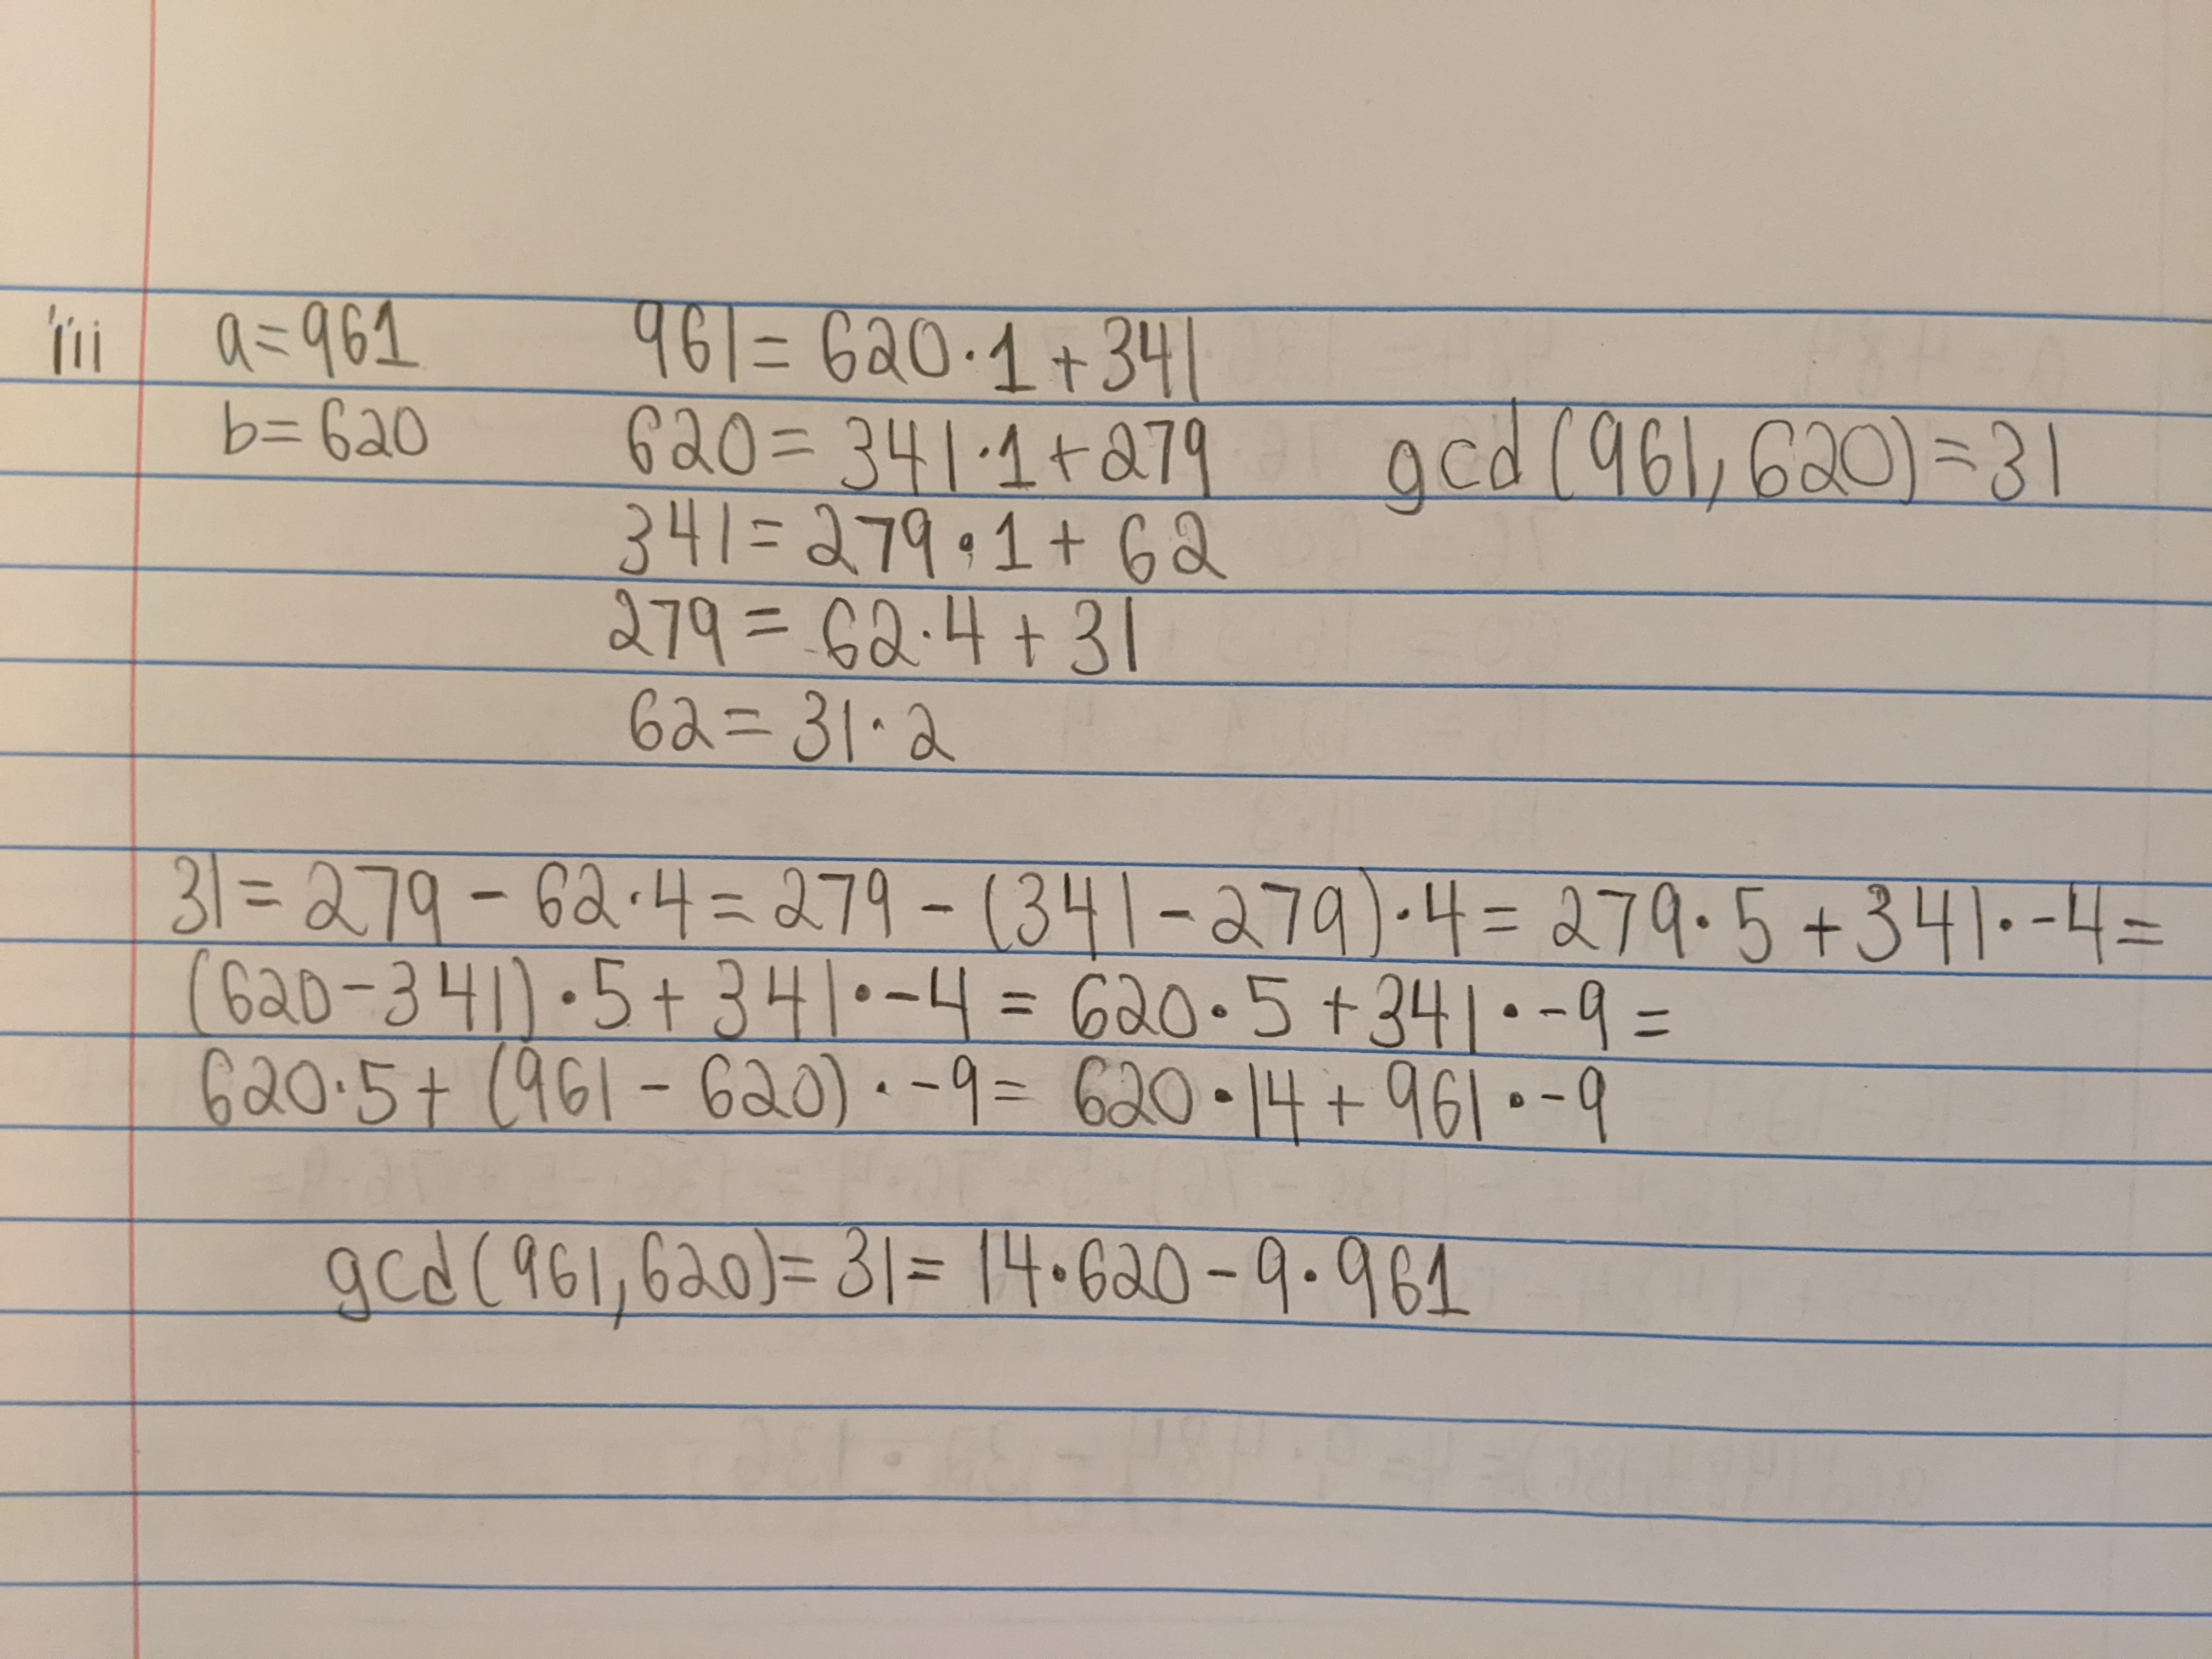
\includegraphics[width=\textwidth]{Problem1Image3}
\end{figure}
\newpage
\section*{Problem 2}
\subsection*{Part (i)}
First, we claim that every integer is even or odd. To prove this, we will first use induction to show that every natural number is even or odd. Let $k = 0$. Notice that $k = 0 = 2\cdot 0$, so $k=0$ is even. Next, we may suppose that $k\geq 0$ is even or odd, and we will show that $k+1$ is even or odd. If $k$ is even, then we may write $k=2n$ for some integer $n$ so that $k+1 = 2n+1$ is odd. If $k$ is odd, then we may write $k = 2n+1$ for some integer $n$ so that $k+1 = 2n+2 = 2(n+1)$ is even. By induction, we have thus shown that every natural number is even or odd. Next, we claim that every negative integer is even or odd. Let $k$ be a negative integer. Then $-k$ is a positive integer, so it is either even or odd. If $-k$ is even, then $-k = 2n$ for some integer $n$ so that $k= 2(-n)$ is even. If $-k$ is odd, then $-k = 2n+1$ for some integer $n$ so that $k = -2n - 1 = 2(-n-1)+1$ is odd. This shows that every negative integer is either even or odd. Thus, we may conclude that every integer is even or odd.
\\ \\
Next, we claim that for every integer $k$, $k(k+1)$ is even. By the above result, we know that $k$ is even or odd. If $k$ is even, then we may write $k = 2n$ for some integer $n$ so that $k(k+1) = 2n(2n+1)= 2(n(2n+1))$ is even. If $k$ is odd, then we may write $k = 2n+1$ for some integer $n$ so that $k(k+1) = (2n+1)(2n+1+1) = (2n+1)(2n+2) = 2((2n+1)(n+1))$ is even. Thus, we know that $k(k+1)$ is even for every integer $k$.
\newpage
\subsection*{Part (ii)}
Since $n$ is assumed to be odd, we know that $n$ is congruent to $1$ or $3$ modulo $4$ (if $n \equiv 0 \pmod{4}$ or $n \equiv 2 \pmod{4}$, then $n$ would be even, contradicting our assumption that $n$ is odd). First, we may suppose that $n \equiv 1 \pmod{4}$ so that $n = 4p + 1$ for some integer $p$. Now, we note that
\[
n^2 - 1 = (4p+1)^2 - 1 = 16p^2 + 8p + 1 - 1 = 16p^2 + 8p = 8(2p^2+p)
\] so that $n^2 - 1$ is divisible by $8$. Next, we may suppose that $n \equiv 3 \pmod{4}$ so that $n = 4p + 3$ for some integer $p$. Then, we obtain
\[
n^2 - 1 = (4p+3)^2 - 1 = 16p^2 + 24p + 9 - 1 = 16p^2 + 24p + 8 = 8(2p^2 + 3p + 1)
\] so that $n^2 - 1$ is divisible by $8$. Thus, we may conclude that $n^2-1$ is divisible by $8$ if $n$ is odd.
\newpage
\section*{Problem 3}
To avoid redundancy in defining the sets $A_1,A_2,A_3,A_4$ below, we will assume throughout this problem that $x > 0$ and $y > 0$ (that is, we are considering the first quadrant of the plane). Furthermore, let $C$ denote the circle of radius $X$ centered at the origin. Now, let us note that
\[
\sum_{1\leq n \leq X} [\sqrt{X^2 -n^2}]
\] is the cardinality of the set
\[
A_1 = \{ (x,y) \in \Z \times \Z: x^2 + y^2 \leq X^2\}
\] That is, it is the number of lattice points in the first quadrant of the plane that are also inside the circle $C$. This is true because for every integer $n$ between $1$ and $X$, $[\sqrt{X^2 - n^2}]$ is the number of lattice points with $x$-coordinate $n$ and positive $y$-coordinate beneath the curve $f(x) = \sqrt{X^2 - x^2}$, which is the equation of the circle $C$.
\\ \\
Next, we note that 
\[
\sum_{1 \leq n \leq X/\sqrt{2}} [\sqrt{X^2 - n^2}]
\]
is the cardinality of the set
\[
A_2 = \{(x,y) \in \Z \times \Z: x \leq X/\sqrt{2}, \; x^2 + y^2 \leq X^2\}
\] That is, it is the number of lattice points in the first quadrant of the plane that are also inside the circle $C$ with the additional property that $x \leq X/\sqrt{2}$. This is true because for every integer $n$ between $1$ and $X/\sqrt{2}$, $[\sqrt{X^2 - n^2}]$ is the number of lattice points with $x$-coordinate $n$ and positive $y$-coordinate beneath the curve $f(x) = \sqrt{X^2 - x^2}$, which is the equation of the circle $C$. Furthermore, we notice that
\[
\sum_{1 \leq n \leq X/\sqrt{2}} [\sqrt{X^2 - n^2}]
\] is also the cardinality of the set
\[
A_3 = \{(x,y) \in \Z \times \Z : y \leq X/\sqrt{2}, \; x^2 + y^2 \leq X^2\}
\] That is, it is the number of lattice points in the first quadrant of the plane that are also inside the circle $C$ with the additional property that $y \leq X/\sqrt{2}$. This is true because for every integer $n$ between $1$ and $X/\sqrt{2}$, $[\sqrt{X^2 - n^2}]$ is the number of lattice points with $y$-coordinate $n$ and positive $x$-coordinate to the left of the curve $f(y) = \sqrt{X^2 - y^2}$, which is the equation of the circle $C$. Finally, we note that 
\[
[X/\sqrt{2}]^2
\] is the cardinality of the set
\[
A_4 = \{(x,y) \in \Z \times \Z: x \leq X/\sqrt{2}, \; y \leq X/\sqrt{2}\}
\] That is, it is the number of lattice points in a square with side length $X/\sqrt{2}$ whose bottom-left corner is at the origin. This is true because $[X/\sqrt{2}]$ is the number of positive integers less than or equal to $X/\sqrt{2}$. Now, we claim that $A_1 = A_2 \cup A_3$ and that $A_2 \cap A_3 = A_4$. First, we will prove that $A_1 = A_2 \cup A_3$. Let $(x,y) \in A_1$. Then, we know that $x^2 + y^2 \leq X^2$. If $(x,y) \not \in A_2 \cup A_3$, then we must have $x > X/\sqrt{2}$ and $y > X/\sqrt{2}$ so that
\[
x^2 + y^2 > \frac{X^2}{2} + \frac{X^2}{2} = X^2
\] contradicting our assumption that $(x,y) \in A_1$. Thus, we know that $(x,y) \in A_2 \cup A_3$ so that $A_1 \subseteq A_2 \cup A_3$. Conversely, we may suppose that $(x,y) \in A_2 \cup A_3$. By the definition of $A_2$ and $A_3$, we know that $x^2+y^2 \leq X^2$ so that $(x,y) \in A_1$. Therefore, we may deduce that $A_2 \cup A_3 \subseteq A_1$, so we know that $A_1 = A_2 \cup A_3$. Next, we claim that $A_2 \cap A_3 = A_4$. First, let $(x,y) \in A_2 \cap A_3$. By definition, we have $x \leq X/\sqrt{2}$ and $y \leq X/\sqrt{2}$, so we know that $(x,y) \in A_4$. Thus, we may deduce that $A_2 \cap A_3 \subseteq A_4$. Conversely, suppose that $(x,y) \in A_4$. Then, we know that $x \leq X/\sqrt{2}$ and $y \leq X/\sqrt{2}$ so that
\[
x^2 + y^2 \leq \frac{X^2}{2} + \frac{X^2}{2} = X^2
\] This informs us that $(x,y) \in A_2 \cap A_3$ so that $A_4 \subseteq A_2 \cap A_3$. Thus, we may deduce that $A_2 \cap A_3 = A_4$. Since $A_1 = A_2 \cup A_3$ and $A_2 \cap A_3 = A_4$, we know that
\[
\vert A_1 \vert = \vert A_2 \cup A_3 \vert = \vert A_2 \vert + \vert A_3 \vert - \vert A_2 \cap A_3 \vert = \vert A_2 \vert + \vert A_3 \vert - \vert A_4 \vert
\] Substituting the appropriate values for $\vert A_1 \vert$, $\vert A_2 \vert$, $\vert A_3 \vert$, $\vert A_4 \vert$, we find that
\[
\sum_{1\leq n \leq X} [\sqrt{X^2 -n^2}] = 2 \Bigg( \sum_{1 \leq n \leq X/\sqrt{2}} [\sqrt{X^2 - n^2}] \Bigg) - [X/\sqrt{2}]^2
\] The intuition behind this solution may be seen in the below image. The set $A_1$ is the union of the red, green, and blue regions, the set $A_2$ is the union of the red and green regions, the set $A_3$ is the union of the green and blue regions, and the set $A_4$ is the green region. Therefore, it is reasonable that the number of lattice points in $A_1$ is equal to the number of lattice points in $A_2$ plus the number of lattice points in $A_3$ minus the number of lattice points in $A_4$ (since we are double-counting the number of lattice points in the green region).
 \begin{figure}[H]
\centering
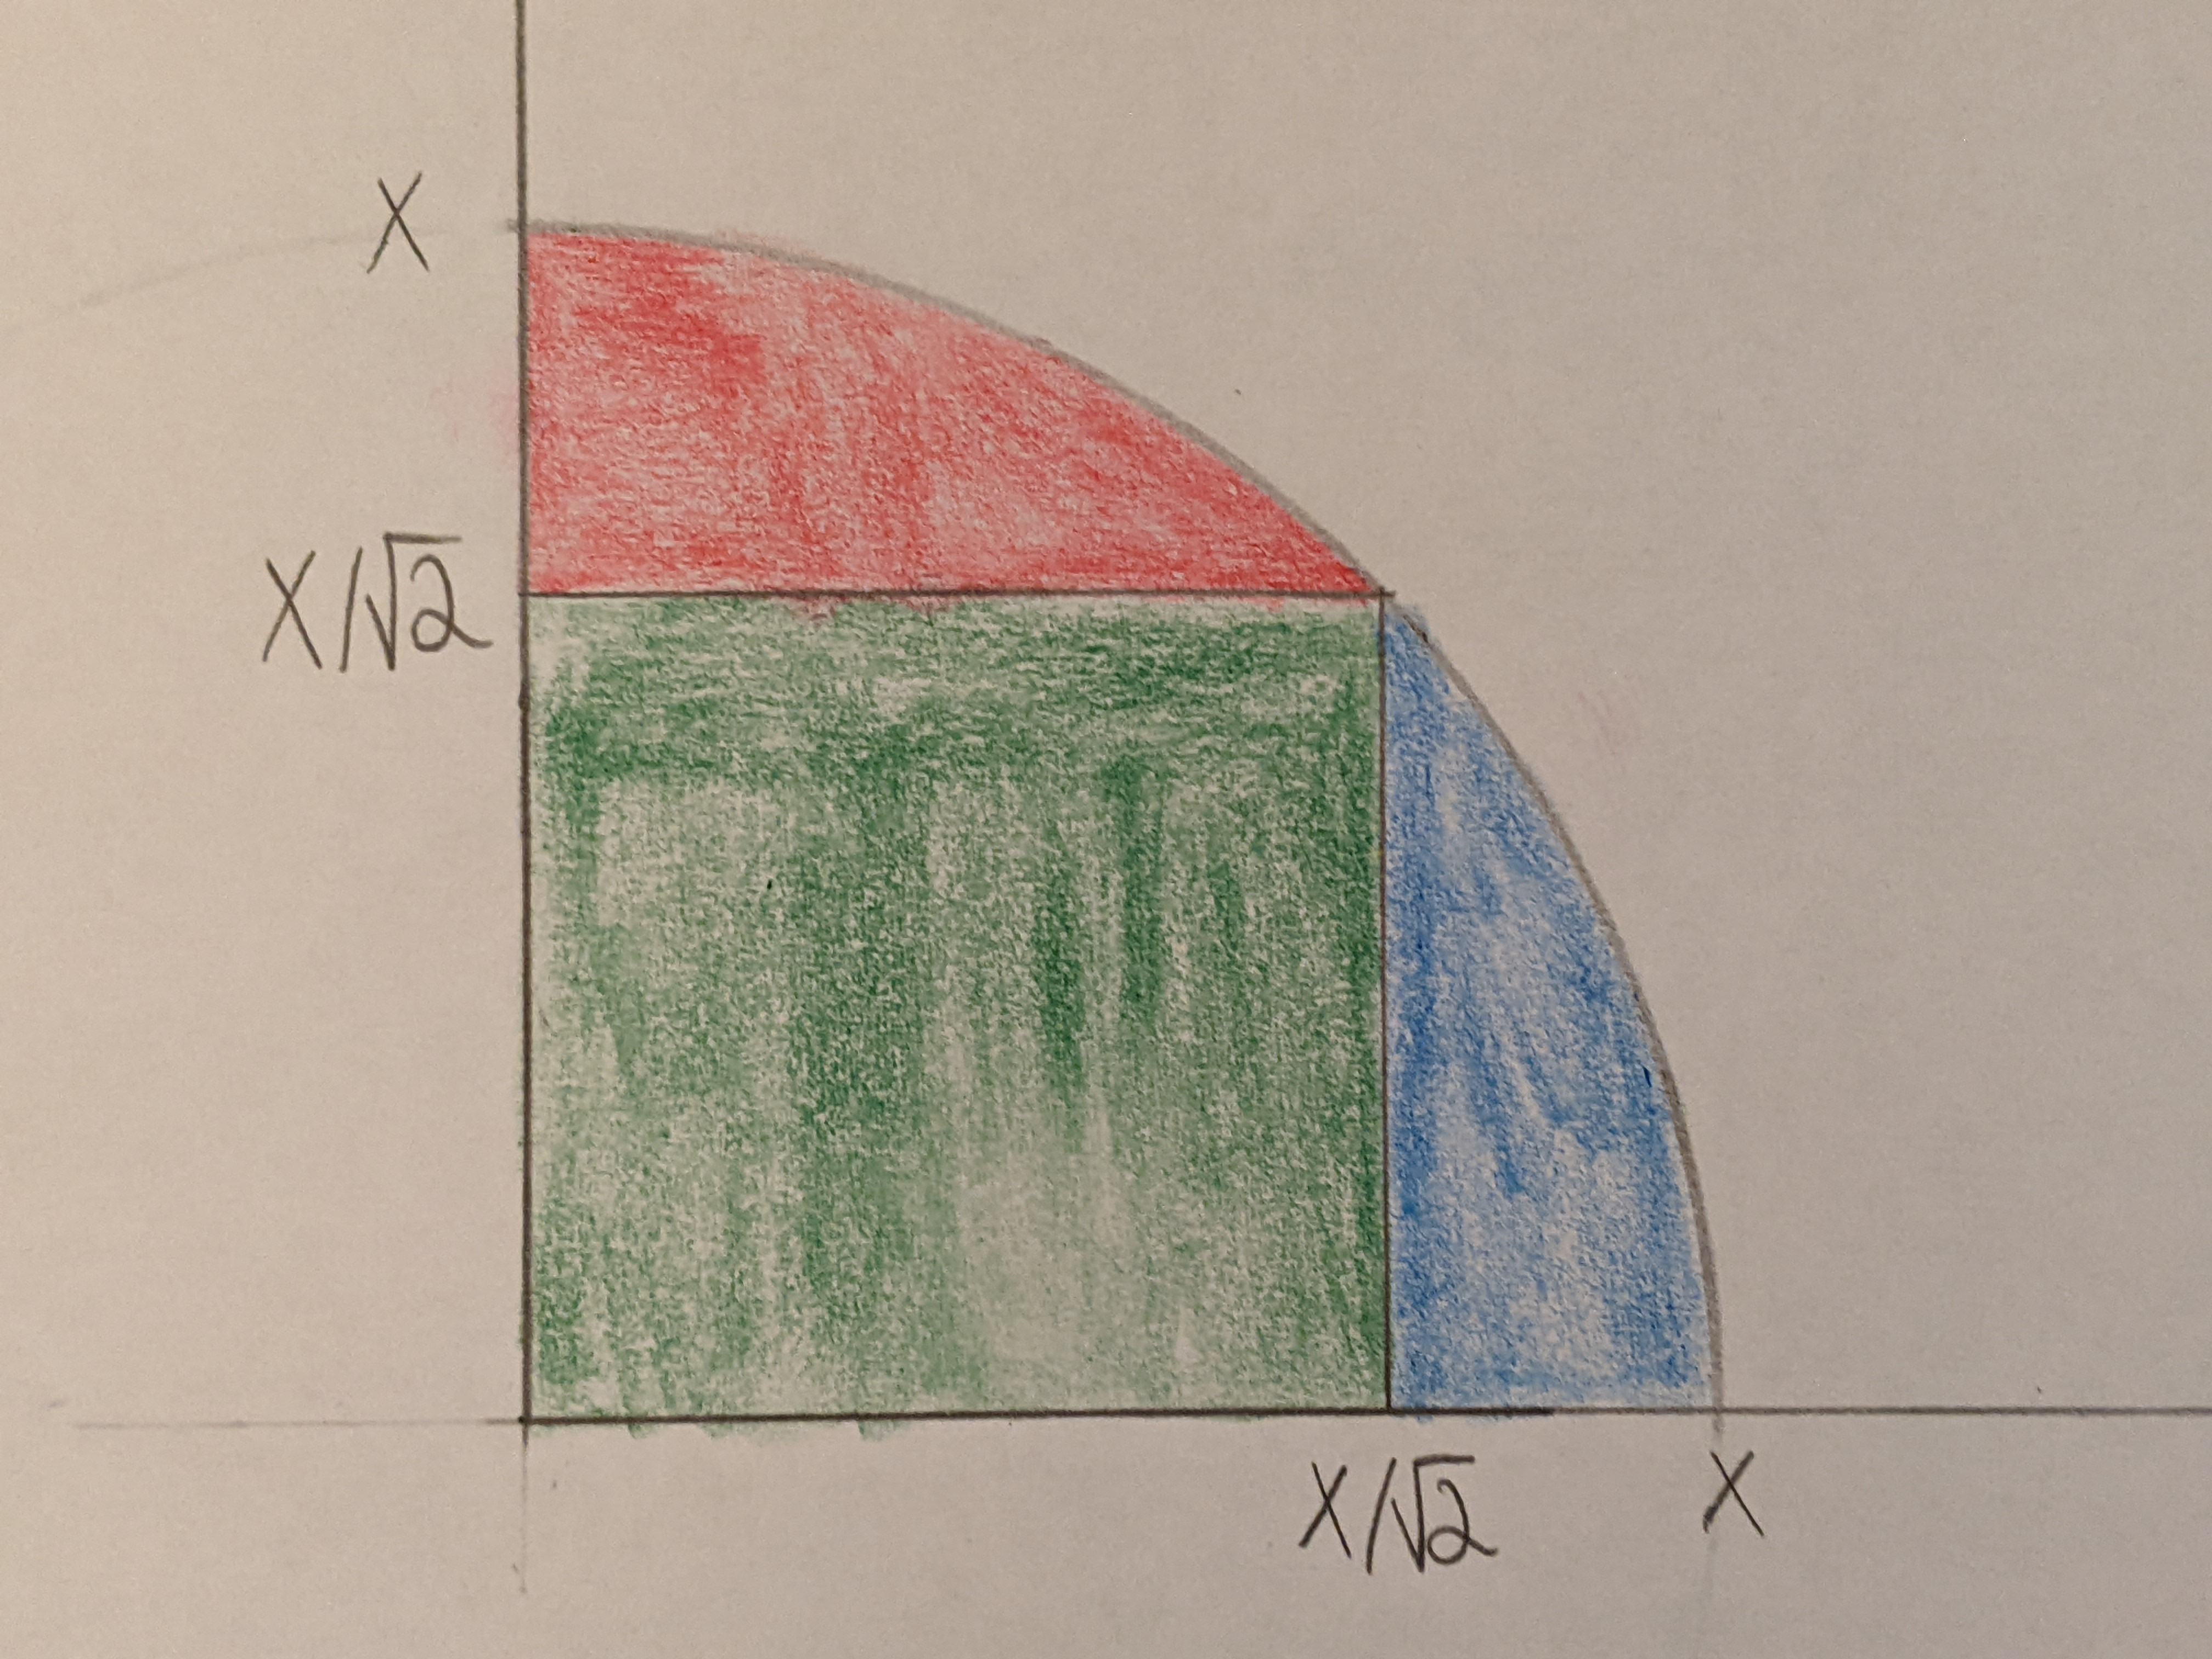
\includegraphics[width=\textwidth]{Problem3Image1}
\end{figure}
\newpage
\section*{Problem 4}
First, we will suppose that $\tau(n)$ is odd. If $\tau(n) = 1$ (so that $n  = 1$), then we know that $1 = 1^2$. Thus we may suppose that $\tau(n) > 1$, which implies that $n > 1$. By the Fundamental Theorem of Arithmetic, we may write $n = q_1^{f_1} \cdots q_l^{f_l}$, where $q_1 < \cdots < q_l$ are distinct primes and $f_1,\ldots, f_l$ are all integers strictly greater than $0$. In class, we proved that
\[
\tau(n) = (f_1+1)\cdots(f_l+1)
\] Thus, we know that $(f_1+1)\cdots (f_l+1)$ is odd. If $(f_i+1)$ is even for any $i$, then the product would be even, so we know that $(f_i+1)$ is odd for all $i$. Therefore, we find that $f_i$ is even for all $i$ so that $f_i/2$ is an integer for all $i$. Then, we may write
\[
n = q_1^{f_1} \cdots q_l^{f_l} = (q_1^{f_1/2})^2 \cdots (q_l^{f_l/2})^2 = (q_1^{f_1/2}\cdots q_l^{f_l/2})^2
\] Thus, we have shown that there exists some integer $k = q_1^{f_1/2}\cdots q_l^{f_l/2}$ such that $n = k^2$.
\\ \\
Conversely, let us suppose that there exists some positive integer $k$ such that $n = k^2$. If $k = 1$, then we have $n = 1$ so that $\tau(n) = 1$ is odd. Thus, we may suppose that $k > 1$, so it has a prime factorization $k = q_1^{f_1} \cdots q_l^{f_l}$, where $q_1 < \cdots < q_l$ are distinct primes and $f_1,\ldots,f_l$ are all integers strictly greater than $0$. Then $n = q_1^{2f_1}\cdots q_l^{2f_l}$ so that
\[
\tau(n) = (2f_1 + 1)\cdots (2f_l + 1)
\] is odd.
\newpage
\section*{Problem 5}
\subsection*{Part (i)}
We may consider this problem by cases. First, let us consider the case in which $n$ is even. We may split this case into two subcases. In the first subcase, we may suppose that $n = 2^{e}$ for some integer $e > 1$ (that is, we assume that the prime decomposition of $n$ only contains factors of $2$; we may assume that $e>1$ because $n > 2$ by assumption). In this case, we have
\[
\varphi(2^{e}) = 2^e - 2^{e-1} = 2^{e-1}(2 - 1) = 2^{e-1}
\] so that $\varphi(n)$ is even (in class, we proved that $\varphi(p^k) = p^k - p^{k-1}$ for any prime $p$ and positive integer $k$).
In the second subcase, we suppose that $n$ has at least one odd prime factor so that we may write $n = 2^{e_1} p_2^{e_2} \cdots p_k^{e_k}$, where $p_2 < \cdots < p_k$ are distinct odd primes and $e_1,\ldots,e_k$ are all integers strictly greater than $0$. Since we proved that $\varphi$ is multiplicative in class, we have
\begin{align*}
&\varphi(n) = \varphi(2^{e_1} p_2^{e_2} \cdots p_k^{e_k}) = \varphi(2^{e_1})\varphi(p_2^{e_2})\cdots\varphi(p_k^{e_k}) = (2^{e_1} - 2^{e_1-1})(p_2^{e_2} - p_2^{e_2 - 1})\cdots (p_k^{e_k} - p_k^{e_k - 1}) \\ &= 2^{e_1 - 1}(2-1)p_2^{e_2 - 1}(p_2 - 1)\cdots p_k^{e_k - 1}(p_k - 1) = 2^{e_1 - 1}p_2^{e_2 - 1}(p_2 - 1)\cdots p_k^{e_k - 1}(p_k - 1)
\end{align*} Since $p_2 - 1$ is even, we find that $\varphi(n)$ is even.
\\ \\
Next, let us consider the case in which $n$ is odd. Then, we may write $n = p_1^{e_1} \cdots p_k^{e_k}$, where $p_1 < \cdots < p_k$ are distinct odd primes and $e_1,\ldots,e_k$ are all integers strictly greater than $0$. As above, we have
\[
\varphi(n) = p_1^{e_1 - 1}(p_1-1)\cdots p_k^{e_k - 1}(p_k - 1)
\] Notice that $p_1 - 1$ is even so that $\varphi(n)$ is even.
\newpage
\subsection*{Part (ii)}
First, notice that since $p_1p_2 \mid n$, $p_1$ and $p_2$ must each divide $n$. Thus, $n$ must contain at least one copy of $p_1$ and $p_2$ in its prime factorization. We may now consider this problem by cases. Let us first consider the case in which $n$ is even. Then, we have $n = 2^{\alpha}p_1^{e_1}p_2^{e_2} \cdots p_k^{e_k}$, where $2 < p_1 < p_2 < \cdots < p_k$ are distinct primes and $\alpha, e_1, e_2, \ldots, e_k$ are all integers strictly greater than $0$. Now, we note that
\begin{align*}
& \varphi(n) = \varphi(2^{\alpha}p_1^{e_1} p_2^{e_2} \cdots p_k^{e_k}) = \varphi(2^\alpha)\varphi(p_1^{e_1})\varphi(p_2^{e_2})\cdots \varphi(p_k^{e_k}) \\ 
& = (2^\alpha - 2^{\alpha - 1})(p_1^{e_1} - p_1^{e_1 - 1})(p_2^{e_2} - p_2^{e_2 - 1})\cdots (p_k^{e_k} - p_k^{e_k - 1})\\
& = 2^\alpha(1-1/2)p_1^{e_1}(1-1/p_1)p_2^{e_2}(1-1/p_2)\cdots p_k^{e_k}(1-1/p_k) \\
& = 2^\alpha p_1^{e_1} p_2^{e_2} \cdots p_k^{e_k} (1-1/2)(1-1/p_1)(1-1/p_2)\cdots(1 - 1/p_k) \\
& = n (1-1/2) (1-1/p_1)(1-1/p_2)\cdots(1 - 1/p_k)
\end{align*} Now, we note that
\begin{align*}
&\frac{n}{\varphi(n)} = \frac{n}{n(1-1/2) (1-1/p_1)(1-1/p_2)\cdots(1 - 1/p_k)} \\
& = \frac{1}{(1-1/2) (1-1/p_1)(1-1/p_2)\cdots(1 - 1/p_k)} = \frac{2p_1p_2\cdots p_k}{(p_1-1)(p_2-1)\cdots(p_k-1)}
\end{align*} In order for $n/\varphi(n)$ to be an integer, we must have
\[
(p_1-1)(p_2-1)\cdots (p_k -1)  \mid 2 p_1 p_2 \cdots p_k
\] Since $p_1$ and $p_2$ are both odd, $p_1-1$ and $p_2 - 1$ must both be even. Thus, we may write $(p_1-1)(p_2-1)\cdots (p_k -1) = 2^a \cdot m$, where $a\geq 2$ and $m$ is odd. Thus, we find that
\[
2^a \cdot m \mid 2 p_1 p_2 \cdots p_k
\] so that
\[
2^{a-1} \cdot m \mid p_1 p_2 \cdots p_k
\] This means that $2$ must divide one of the odd primes $p_1,p_2,\ldots, p_k$. Thus, $2$ must be equal to one of the odd primes $p_1,p_2,\ldots,p_k$. This is impossible since $2$ is even.
\\ \\
Next, we may consider the case in which $n$ is odd. Then, we have $n = p_1^{e_1} p_2^{e_2} \cdots p_k^{e_k}$, where $p_1 < p_2 < \cdots < p_k$ are distinct odd primes and $e_1,e_2,\ldots,e_k$ are all integers strictly greater than $0$. Now, we note that
\begin{align*}
& \varphi(n) = \varphi(p_1^{e_1} p_2^{e_2} \cdots p_k^{e_k}) = \varphi(p_1^{e_1}) \varphi(p_2^{e_2}) \cdots \varphi(p_k^{e_k}) = (p_1^{e_1} - p_1^{e_1 - 1})(p_2^{e_2} - p_2^{e_2-1})\cdots (p_k^{e_k} - p_k^{e_k - 1})\\
& = p_1^{e_1}(1-1/p_1)p_2^{e_2}(1-1/p_2) \cdots p_k^{e_k}(1-1/p_k) = p_1^{e_1} p_2^{e_2} \cdots p_k^{e_k} (1-1/p_1)(1-1/p_2)\cdots(1 - 1/p_k) \\
&= n (1-1/p_1)(1-1/p_2)\cdots(1 - 1/p_k)
\end{align*} Now, we note that
\begin{align*}
&\frac{n}{\varphi(n)} = \frac{n}{n (1-1/p_1)(1-1/p_2)\cdots(1 - 1/p_k)} = \frac{1}{(1-1/p_1)(1-1/p_2)\cdots(1 - 1/p_k)} \\
&= \frac{p_1p_2\cdots p_k}{(p_1 - 1)(p_2 - 1)\cdots(p_k - 1)}
\end{align*} 
In order for $n/ \varphi(n)$ to be an integer, we must have
\[
(p_1 - 1)(p_2 - 1) \cdots (p_k - 1) \mid p_1 p_2 \cdots p_k
\] Since $p_1$ and $p_2$ are both odd, $p_1 - 1$ and $p_2 - 1$ are both even. Thus, we may write $(p_1-1)(p_2 - 1) \cdots (p_k - 1) = 2^a \cdot m$, where $a \geq 2$ and $m$ is odd. We find that
\[
2^a \cdot m \mid p_1 p_2 \cdots p_k
\] so that $2$ must divide some odd prime $p_1,p_2,\ldots,p_k$. This can only occur if $2$ is equal to one of $p_1,p_2,\ldots,p_k$. This is impossible since $2$ is even.
\end{document} 